% \iffalse meta-comment
%<*internal>
\def\nameofplainTeX{plain}
\ifx\fmtname\nameofplainTeX\else
\expandafter\begingroup
\fi
%</internal>
%
%
%
%
% ^^A -------------------------------------- .ins -------------------------------------
%<*install>
\input docstrip.tex
\keepsilent
\askforoverwritefalse
\preamble
----------------------------------------------------------------
utfpr-pg --- Classe para trabalhos acadêmicos da UTFPR-PG
Author:  Fabiano Rosas, Gabriel Casella
E-mail:  fabianorosas@gmail.com, gbc921@gmail.com
License: Released under the LaTeX Project Public License v1.3c or later
See:     http://www.latex-project.org/lppl.txt
----------------------------------------------------------------
\endpreamble

\postamble
Customizations of the abnTeX2 class (http://abnTeX2.googlecode.com)

This work may be distributed and/or modified under the
conditions of the LaTeX Project Public License (LPPL), either
version 1.3c of this license or (at your option) any later
version.  The latest version of this license is in the file:

http://www.latex-project.org/lppl.txt

This work is "maintained" (as per LPPL maintenance status) by
(not set).

This work consists of the file utfpr-pg.dtx and a Makefile.
Running make generates the derived files README.txt, utfpr-pg.pdf and utfpr-pg.cls.
Running make inst installs the files in the user's TeX tree.
Running make install installs the files in the local TeX tree.

Further information about abnTeX2 is available on http://abntex2.googlecode.com/
\endpostamble

\usedir{tex/latex/utfpr-pg}
\generate{
        \file{\jobname.cls}{\from{\jobname.dtx}{class}}
        \file{\jobname.bib}{\nopreamble\nopostamble\from{\jobname.dtx}{bibliography}}
}
%</install>
%<install>\endbatchfile
%<*internal>
\usedir{source/latex/utfpr-pg}
\generate{
        \file{\jobname.ins}{\from{\jobname.dtx}{install}}
}
\ifx\fmtname\nameofplainTeX
\expandafter\endbatchfile
\else
\expandafter\endgroup
\fi
%</internal>
% \fi
%
%
%
%
% ^^A---------------------------------------------- .dtx ----------------------------------------
% \iffalse
%<*driver>
\ProvidesFile{utfpr-pg.dtx}
%</driver>
%<class>\NeedsTeXFormat{LaTeX2e}[1999/12/01]
%<class>\ProvidesClass{utfpr-pg}
%<*class>
[2013/10/30 v1.00 Classe para trabalhos acadêmicos da UTFPR-PG]
%</class>
%<class>\DeclareOption*{\PassOptionsToClass{\CurrentOption}{abntex2}}
%<class>\ProcessOptions\relax
%<*driver>
\documentclass{ltxdoc}
\usepackage[a4paper,margin=25mm,left=50mm,nohead]{geometry}
\usepackage[numbered]{hypdoc}
\usepackage[utf8]{inputenc}
\usepackage[T1]{fontenc}
\usepackage{xcolor}
\usepackage{pbox}
\usepackage{url}
\usepackage{subcaption}
\usepackage{graphicx}
\usepackage[within=none]{newfloat}
\usepackage[font=itshape]{quoting}
\usepackage[brazil]{babel}
\usepackage[alf,abnt-emphasize=bf,abnt-repeated-author-omit=yes]{abntex2cite}
\definecolor{dark-gray}{gray}{0.20}
\definecolor{light-gray}{gray}{0.85}

\newcommand{\com}[1]{
        \colorbox{light-gray}{\texttt{\pbox{\textwidth}{\$ #1}}}
}

\newcommand{\cominline}[1]{
        \colorbox{light-gray}{\texttt{\pbox{\textwidth}{#1}}}
}

\newcommand\linha{\leavevmode\xleaders\hbox{-}\hfill\kern0pt}

\DeclareFloatingEnvironment[
fileext=loq,
listname=Lista de Quadros,
name=Quadro,
placement=tbhp,
]{quadro}

\EnableCrossrefs
%^^A\CodelineIndex
\begin{document}
\DocInput{\jobname.dtx}
\end{document}
%</driver>
% \fi
%
% \GetFileInfo{\jobname.dtx}
% \DoNotIndex{\newcommand,\newenvironment,\center,\com,\cominline}
%
% \title{\textsf{utfpr-pg} --- Classe para trabalhos acadêmicos da UTFPR-PG.}
%
% \author{Fabiano Rosas\\Gabriel Casella\thanks{fabianorosas@gmail.com, gbc921@gmail.com}}
% \date{Released \filedate}
%
% \maketitle
%
%
% \begin{abstract}
%   Com o intuito de aproveitar as facilidades introduzidas pela classe abn\TeX2 para a formatação de trabalhos acadêmicos de acordo com as normas da \textbf{ABNT} está sendo desenvolvida a classe \textsf{utfpr-pg}, que implementa as normas de formatação de trabalhos acadêmicos da Universidade Tecnológica Federal do Paraná, campus Ponta Grossa.
% \end{abstract}
%
%
%
% \section{Obtenção}
% \label{sec:obtencao}
%
% A obtenção da classe pode ser feita através do link: TODO:colocar link
%
%
%
% \section{Instalação}
% \label{sec:instalacao}
%
% Para a instalação é necessário estar de posse dos arquivos \jobname.dtx e Makefile.
%
% Utilize \cominline{make} para gerar os arquivos README.txt, utfpr-pg.pdf and utfpr-pg.cls.
% Em seguida utilize \cominline{make inst} para instalar os arquivos da classe para o usuário.
%
% Para instalar para todos os usuários, utilize \cominline{make install}.
%
% \StopEventually{
% \PrintIndex
% }
%
%
%
% \section{Utilização}
% Depois que os arquivos estiverem nos lugares corretos, a utilização da classe é feita\ldots (TODO: explicar como carregar a classe)
%
%\iffalse ^^A inicia a classe, mas não mostra a tag no pdf
%<*class>
%\fi
%
%
%
% \section{As normas da UTFPR}
% A implementação das normas para trabalhos acadêmicos da UTFPR-PG está sendo feita tomando por base % a classe abn\TeX2 \url{http://abntex2.googlecode.com/}.
%    \begin{macrocode}
\LoadClass[a4paper]{abntex2}
%    \end{macrocode}
% Sendo necessária também a citação na forma alfanumérica da ABNT. O parâmetro |abnt-emphasize=bf| foi adicionado para deixar a ênfase das referências, mais próxima do que é feito mais usualmente, embora a ênfase padrão (itálico) também seja permitida pela norma:
%    \begin{macrocode}
\RequirePackage[alf,abnt-emphasize=bf,abnt-repeated-author-omit=yes]{abntex2cite}
%    \end{macrocode}
% Para identação de todos os parágrafos utiliza-se o pacote \texttt{identfirst}.
%    \begin{macrocode}
\RequirePackage{indentfirst}
%    \end{macrocode}
% A codificação utf-8 é requerida para o funcionamento da classe abn\TeX2.
%    \begin{macrocode}
\RequirePackage[utf8]{inputenc}
%    \end{macrocode}
% O pacote |lastpage| é utilizado na folha de aprovação.
%    \begin{macrocode}
\RequirePackage{lastpage}
%    \end{macrocode}
%
%
%
% \section{Comandos pré-definidos (macros)}
% Além dos comandos padrões da abn\TeX2, como por exemplo, |\autor|, |\titulo| e |\local|, a classe da UTFPR define as seguintes macros:
%
% \DescribeMacro{\utfpr}
% Insere o texto ``Universidade Tecnológica Federal Do Paraná''.
%
% \DescribeMacro{\curso}
% Usa-se para definir o curso de graduação ou especialização.
%
% \DescribeMacro{\departamento}
% Usa-se para definir o departamento, coordenação ou programa.
%
% \DescribeMacro{\novalistade}
% Cria novas listas como lista de quadros ou graficos. Recebe dois parametros obrigatorios. \marg{lista} que define o tipo de lista a ser criado e \marg{ext} que define a extensao de arquivo a ser usada para guardar a lista.
%
% Ex: |\novalistade{quadro}{loq}| criara uma lista de quadros a ser armazenada em um arquivo com a extensao .loq
%
% O comando |\novalistade| ainda define um ambiente para ser usado da mesma forma que |figure| ou |table|.
%
% \DescribeMacro{\listof...} Exibe a lista criada com o comando descrito acima.
%
%\iffalse
\newcommand\utfpr{Universidade Tecnológica Federal Do Paraná}
\newcommand*\erro[1]{\@latex@error{Defina \noexpand#1!}\@ehc}

\providecommand\imprimircurso{\erro\curso}
\newcommand*\curso[1]{\renewcommand{\imprimircurso}{#1}}

\providecommand\imprimirdepartamento{}
\newcommand*\departamento[1]{\renewcommand{\imprimirdepartamento}{#1}}
%\fi
%
%
%
% \section{Ambientes}
% O pacote |newfloat| provê funcionalidades para a criação de novos ambientes flutuantes.
%    \begin{macrocode}
\RequirePackage[within=none]{newfloat}
%    \end{macrocode}
%
% \DescribeMacro{\listadequadros}
% A classe UTFPR-PG provê o ambiente \textsf{Quadro} e o comando |\listadequadros|
%
% Outros ambientes podem ser criados pelo usuário seguindo o seguinte modelo:
%    \begin{macrocode}
\DeclareFloatingEnvironment[
fileext=loq,
listname=Lista de Quadros,
name=Quadro,
placement=tbhp,
]{quadro}
%    \end{macrocode}
% A utilização dos novos ambientes é feita da mesma maneira que o ambiente \textsf{figure}, por exemplo:
% \begin{quadro}
% \begin{center}
%  \linha\par
%
%  $\vert$\hfill Isto não é um quadro\hfill $\vert$
%
% \linha
% \end{center}
% \caption{Exemplo de ambiente}
% \end{quadro}
%
%
%
% \section{Capa}
% Um ponto onde há diferenças visíveis entre as normas da ABNT e as normas da UTFPR é a capa. O livreto de normas da UTFPR, cita que a capa é:
%
% \begin{quoting}
%   elemento obrigatório, proteção externa que reveste o trabalho. Na capa devem constar informações de identificação da obra:
%   \begin{itemize}
%   \item nome da Instituição e do Curso, completos;
%   \item nome do autor(es): responsável intelectual ou artístico do trabalho;
%   \item título principal do trabalho: claro, preciso, com palavras que identifiquem o seu conteúdo;
%   \item subtítulo (se houver): deve ser evidenciada a sua subordinação ao título principal, precedido de dois pontos (:);
%   \item número de volume (se houver mais de um deve constar, em cada capa, a especificação do respectivo volume);
%   \item tipo de documento científico ou acadêmico (tese, dissertação, trabalho de conclusão de curso, monografia de especialização, relatório de pesquisa, ou tros trabalhos acadêmicos);
%   \item local (cidade) da Instituição onde o trabalho deve ser apresentado;
%   \item ano de depósito (entrega do trabalho).
%   \end{itemize}
% \end{quoting}
%
% Para exibir a capa, utiliza-se o comando |\imprimircapa|.
% \begin{macro}{\imprimircapa}
%   A macro |\imprimircapa| da classe abn\TeX2 imprime um modelo básico de capa que atende aos requisitos da seção 4.1.1 da ABNT NBR~14724:2011. A capa não é incluída no bookmark do PDF.
%
%^^A   Esta macro foi redefinida para atender às necessidades da UTFPR-PG:
%^^A    \begin{macrocode}
%\iffalse
\renewcommand{\imprimircapa}{
        \begin{capa}
          \center
          {\large\MakeUppercase\utfpr}\par
          {\large\MakeUppercase\imprimirdepartamento}\par
          {\large\MakeUppercase\imprimircurso}\par
          \vfill
          {\large\MakeUppercase\imprimirautor}\par
          \vfill
          {\bfseries\large\MakeUppercase\imprimirtitulo}\par
          \vfill
          {\large\MakeUppercase\imprimirtipotrabalho}\par
          \vfill
          {\large\MakeUppercase\imprimirlocal}\par
          {\large\imprimirdata}\par
        \end{capa}
}
%\fi
%^^A    \end{macrocode}
% \end{macro}
%
%
%
% \section{Fonte}
% A norma da ABNT não especifica um tipo de fonte a ser utilizado, porém as normas da UTFPR-PG sugerem que para o uso com \LaTeX\ seja utilizada a fonte Nimbus. O pacote \textit{Gyre Termes} implementa as fontes da família Nimbus Roman No 9 L.
%    \begin{macrocode}
\RequirePackage{tgtermes}
%    \end{macrocode}
%
% Para as legendas das ilustrações e tabelas, é necessário o tipo negrito e recomenda-se o uso de fonte tamanho 10. Também é utilizado como largura máxima da legenda a mesma da ilustração ou tabela.
%    \begin{macrocode}
\RequirePackage[font=small,font=bf,labelfont=bf]{caption}
%    \end{macrocode}
% ^^A ajuste das fontes do capitulo e seção
%\iffalse
\renewcommand{\ABNTEXchapterfont}{\bfseries}
\renewcommand{\ABNTEXchapterfontsize}{\normalsize}
\renewcommand{\ABNTEXsectionfont}{}
\renewcommand{\ABNTEXsectionfontsize}{\normalsize}
%^^A\newcommand{\primeirasmaiusculas}[1]{\titlecap{#1}}
%^^A\setsubsecheadstyle{\primeirasmaiusculas}
\renewcommand{\ABNTEXsubsectionfontsize}{\normalsize}
\renewcommand{\ABNTEXsubsubsubsectionfont}{\itshape}
%\fi
%
%
%
% \section{Espaçamentos}
% O espaçamento entre o título do capítulo e o início do texto utilizado pela abn\TeX não é previsto pela ABNT. Para utilizar o espaçamento padrão, o comando a seguir é inserido.
%    \begin{macrocode}
\setlength\afterchapskip{\lineskip}
%    \end{macrocode}
%
% Com relação à indentação inicial do parágrafo, é recomendado utilizar de 1,5 a 2,5 cm. O valor definido por padrão é 1,5 cm. Para modificar este valor, basta utilizar o comando |\setlength| no preâmbulo do documento:
%    \begin{macrocode}
\setlength\parindent{1.5cm}  
%    \end{macrocode}
%
%
%
% \section{Margens}
% Para modificar o tamanho das margens, pode-se utilizar o comando a seguir:
%    \begin{macrocode}
\setlrmarginsandblock{3cm}{2cm}{*}
\setulmarginsandblock{3cm}{2cm}{*}
\checkandfixthelayout
%    \end{macrocode}
%
%
%
% \section{Sumário}
% As modificações feitas para acomodar as normas referentes ao sumário estão listadas a seguir.
%
% \subsection{Espaçamento}\label{s:esp}
% As entradas do sumário estão sendo ajustadas de maneira dinâmica para evitar o problema que ocorre quando a numeração de uma seção fica muito grande e sobrepõe o texto. Na figura \ref{f:sumariotruncado}, o espaçamento entre o número do capítulo e a palavra ``capítulo'' está correto, porém, conforme as seções vão ramificando ou os números aumentando, a visualização vai ficando truncada. O comportamento correto é o apresentado na figura \ref{f:sumariocorreto}.
% \begin{figure}[h]
%   \centering
%   \begin{subfigure}[b]{0.4\textwidth}
%     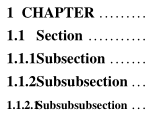
\includegraphics[scale=.95]{imagens/sumariotruncado.png}
%     \caption{Incorreto}
%     \label{f:sumariotruncado}
%   \end{subfigure}
%   \begin{subfigure}[b]{0.4\textwidth}
%     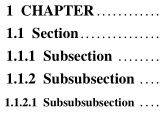
\includegraphics{imagens/sumariocorreto.png}
%     \caption{Correto}
%     \label{f:sumariocorreto}
%   \end{subfigure}
%   \caption{Apresentação do sumário}
% \end{figure}
%
% O ajuste das entradas foi feito alterando a macro |\numberline| que é a responsável por exibir o número da seção (1.1, 1.2.1, etc\ldots) de forma que o tamanho da caixa onde fica o número seja ajustado de acordo com o tamanho que o número ocupa:
%    \begin{macrocode}
\newlength{\@numwidth}
\renewcommand{\numberline}[1]{%
        \settowidth{\@numwidth}{#1}
        \addtolength{\@numwidth}{0.5em}
        \hb@xt@\@numwidth{\@cftbsnum #1\@cftasnum\hfil}\@cftasnumb}
\renewcommand{\chapternumberline}{\numberline}
%    \end{macrocode}
% além disso, é necessário zerar a identação das entradas:
%    \begin{macrocode}
\renewcommand{\tocprintchapter}{
        \addtocontents{toc}{\cftsetindents{chapter}{0em}{1em}}}
\cftsetindents{chapter}{0em}{1em} % here for backwards compatibility, the corret way is the above
\setlength{\cftsectionindent}{0em}
\setlength{\cftsubsectionindent}{0em}
\setlength{\cftsubsubsectionindent}{0em}
%    \end{macrocode}
%
% \subsection{Formatação}
% A formatação das entradas do sumário deve ser feita seguindo a imagem \ref{f:sumario}, ignorando-se as discrepâncias com relação ao espaçamento, que já foram corrigidas na seção \ref{s:esp}.
%\begin{figure}[h]
%  \centering
%  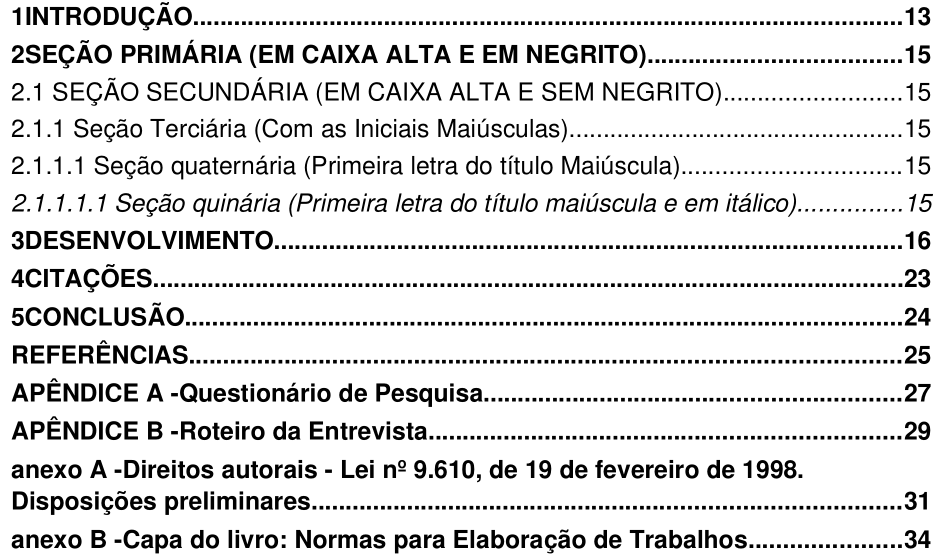
\includegraphics[scale=.3]{imagens/sumario.png}
%  \caption{Sumário de acordo com o livreto de normas da UTFPR}
%  \label{f:sumario}
%\end{figure}
%
% Para remover o espaço entre os capítulos:
%    \begin{macrocode}
\setlength\cftbeforechapterskip{0cm}
%    \end{macrocode}
%
% Ajustes das fontes, capitalização, pesos, etc.
%    \begin{macrocode}
\renewcommand{\cftchapterfont}{\bfseries}
\renewcommand{\cftchapterleader}{\normalfont\cftdotfill{\cftchapterdotsep}}
\renewcommand{\cftchapterpagefont}{\normalfont}
\renewcommand{\cftdotsep}{1}
\newcommand{\upcase}[1]{\uppercase{#1}}
\renewcommand{\cftsectionfont}{\mdseries\upcase}
\renewcommand{\cftsubsectionfont}{\mdseries}
\renewcommand{\cftsubsubsectionfont}{\mdseries}
%    \end{macrocode}
% 
% Fazer com as referências apareçam como um capítulo normal no sumário.
%    \begin{macrocode}
\renewcommand{\bibsection}{\chapter*{\bibname}\prebibhook}
%    \end{macrocode}
%
%
%
%\iffalse ^^A finaliza a tag classe, mas nao mostra no pdf
%</class>
%\fi
%\iffalse ^^A evita que o conteudo do .bib apareça no pdf
% ^^A -------------------------------------- .bib -------------------------------------
%<*bibliography>
@misc{nimbus,
        title = {Nimbus Roman},
        author = {The {LaTeX} Font Catalogue},
        url = {http://www.tug.dk/FontCatalogue/nimbus/},
        urldate = {2013-11-01},
        year = {2013},
        file = {The LaTeX Font Catalogue – Nimbus Roman:/home/fabiano/.zotero/zotero/ru3nfjod.default/zotero/storage/2I5F789D/nimbus.html:text/html}
},

@misc{gyre,
        title = {{TeX} Gyre Termes},
        author = {The {LaTeX} Font Catalogue – },
        url = {http://www.tug.dk/FontCatalogue/tgtermes/},
        urldate = {2013-11-01},
        year = {2013},
        file = {The LaTeX Font Catalogue – TeX Gyre Termes:/home/fabiano/.zotero/zotero/ru3nfjod.default/zotero/storage/FAVQWTBI/tgtermes.html:text/html}
}

@misc{abntex2,
        title = {A classe abntex2: Documentos técnicos e científicos brasileiros compatíveis com as normas ABNT},
        author = {Lauro César Araújo},
        url = {http://ctan.tche.br/macros/latex/contrib/abntex2/doc/abntex2.pdf},
        year = {2014}
}

@manual{memoir,
  title = {The Memoir Class},
  author = {Peter Wilson},
  month = {Abril},
  year = {2013},
  owner = {fabiano},
  timestamp = {2014.02.24},
  url = {http://repositorios.cpai.unb.br/ctan/macros/latex/contrib/memoir/memman.pdf}
}

@manual{latex2e,
  title = {LaTeX2e for class and package writers},
  organization = {The LaTeX 3 Project},
  month = {Março},
  year = {1999},
  owner = {fabiano},
  timestamp = {2014.02.24},
  url = {http://latex-project.org/guides/clsguide.pdf}
}

@manual{package,
  title = {How to package your LaTeX package},
  author = {Scott Pakin},
  month = {Novembro},
  year = {2004},
  owner = {fabiano},
  timestamp = {2014.02.24},
  url = {http://www.tex.ac.uk/ctan/info/dtxtut/dtxtut.pdf}
}

@manual{abntex2cite,
  title = {O pacote abntex2cite: Estilos bibliográficos compatíveis com a ABNT NBR 6023},
  author = {Lauro César Araújo},
  month = {Janeiro},
  year = {2014},
  owner = {fabiano},
  timestamp = {2014.02.24},
  url = {http://repositorios.cpai.unb.br/ctan/macros/latex/contrib/abntex2/doc/abntex2cite.pdf}
}

%</bibliography>
%\fi
%
%
% \nocite{abntex2cite}
% \nocite{package}
% \nocite{latex2e}
% \nocite{memoir}
% \nocite{abntex2}
% \nocite{gyre}
% \nocite{nimbus}
% \bibliography{utfpr-pg}
%
%
\endinput
% \Finale
